% Figure 4.2 (Session 4): what crosses a cut, from two spins to a matrix product state and a lattice.
% The image is rendered by figures/blender/s4_2_schmidt_cut.py; the coordinates of the labels come
% from figures/blender/out/schmidt_cut_anchors.tex. Compile with:
%   pdflatex schmidt_cut.tex ; result moves to ../mps_spin_chains/schmidt_cut.pdf
\documentclass[11pt,tikz,border=0pt]{standalone}
\usepackage{amsmath,amssymb,graphicx}
\usepackage{xcolor}
\definecolor{coursedark}{HTML}{1B2A4A}
\definecolor{costamber}{HTML}{B8620A}
\newlength{\figw}\setlength{\figw}{16.19cm}   % the text width of the notes (letter, 2.7 cm margins), so labels print at size

\begin{document}
\begin{tikzpicture}[lbl/.style={font=\small, text=coursedark}]
  \node[anchor=south west, inner sep=0pt] at (0,0)
    {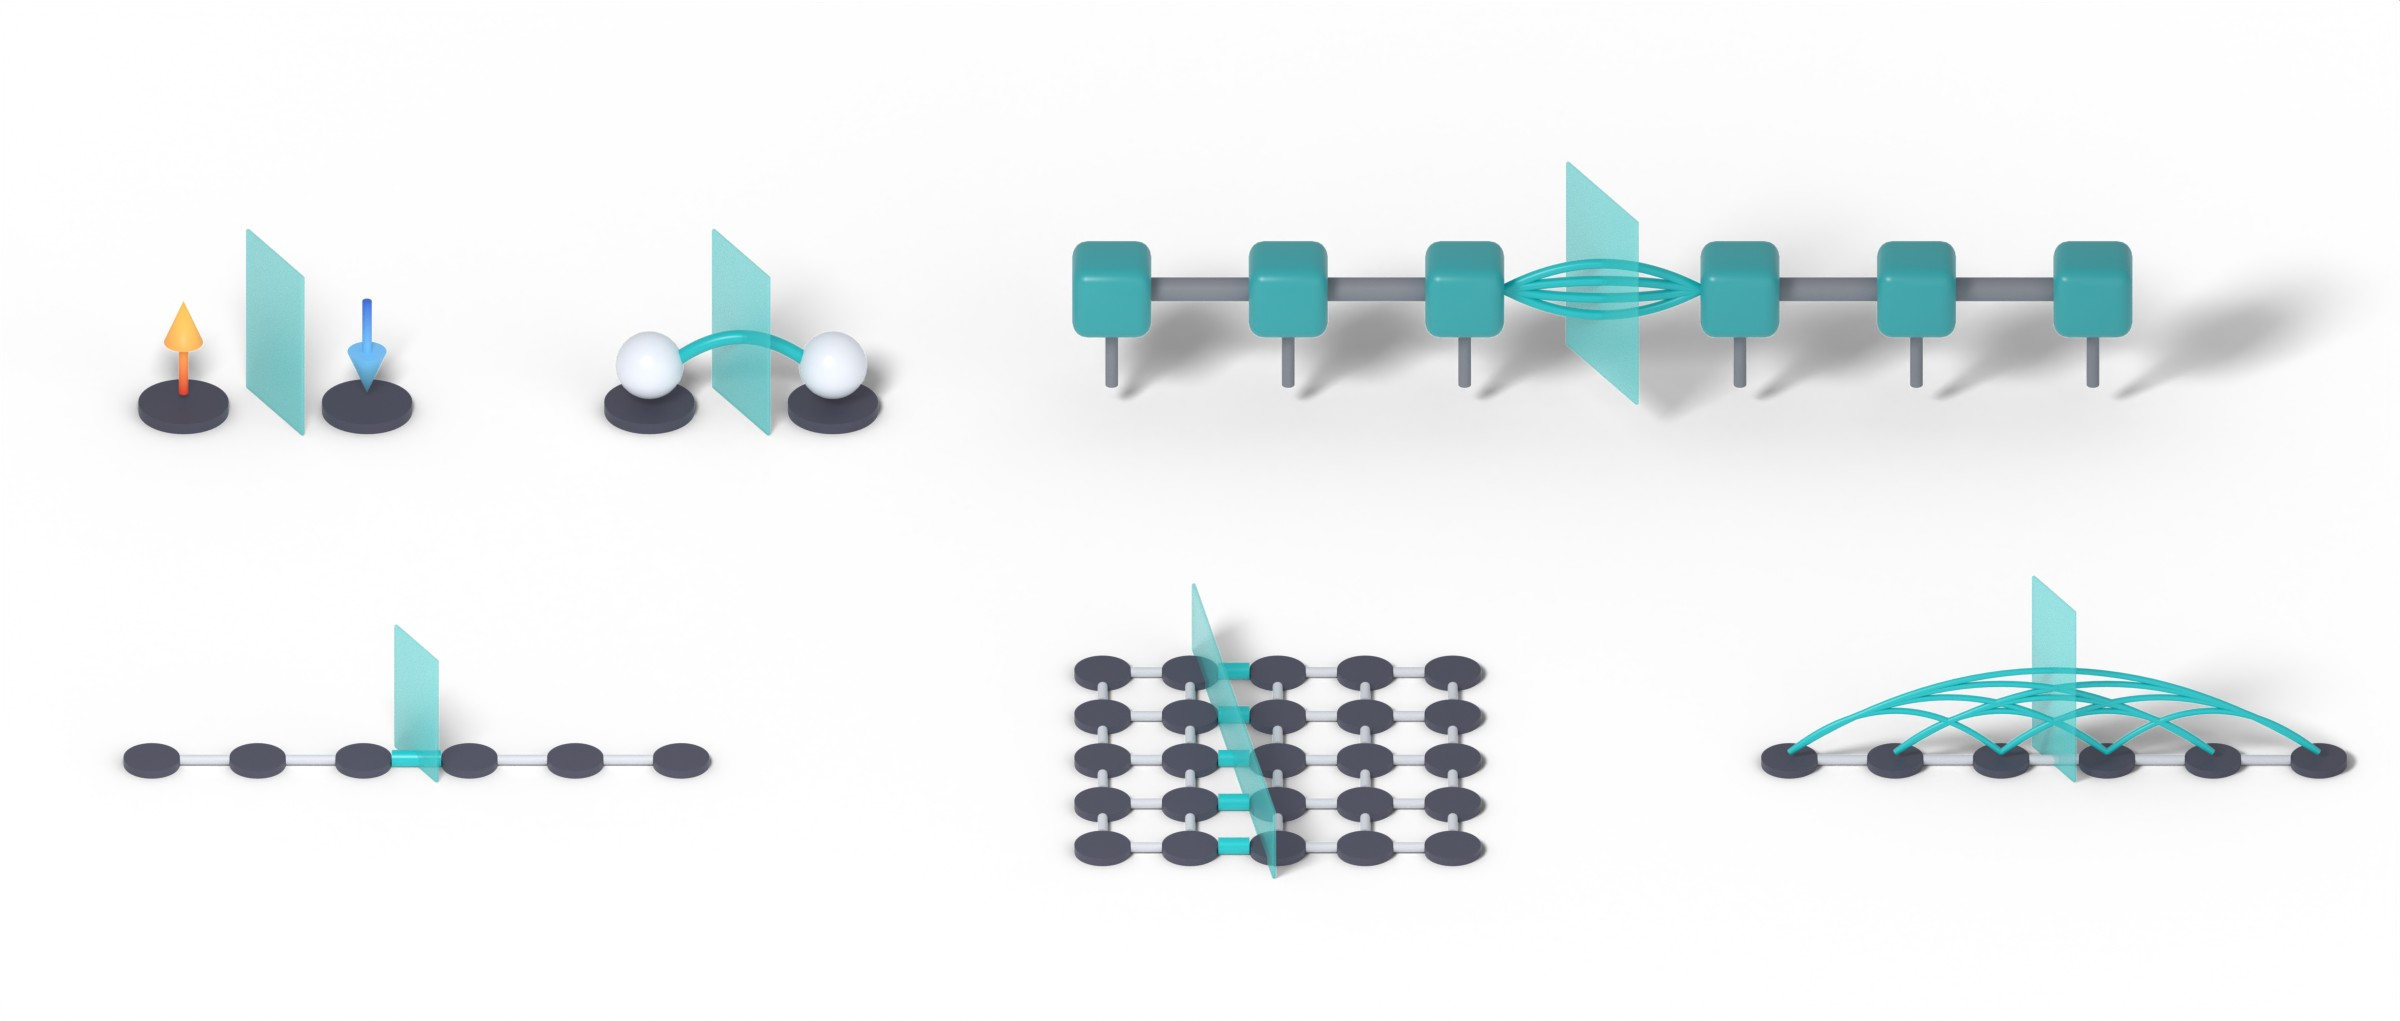
\includegraphics[width=\figw]{../blender/out/schmidt_cut.jpg}};
  %% written by figlib.py; x and y in units of the image width
\coordinate (a) at (0.0118\figw,0.3940\figw);
\coordinate (prod) at (0.1147\figw,0.3278\figw);
\coordinate (sing) at (0.3088\figw,0.3278\figw);
\coordinate (b) at (0.4221\figw,0.3940\figw);
\coordinate (blockA) at (0.5368\figw,0.3329\figw);
\coordinate (blockB) at (0.7985\figw,0.3329\figw);
\coordinate (chin) at (0.6676\figw,0.3583\figw);
\coordinate (sn) at (0.6103\figw,0.2539\figw);
\coordinate (sn1) at (0.7250\figw,0.2539\figw);
\coordinate (s1) at (0.4632\figw,0.2539\figw);
\coordinate (sL) at (0.8721\figw,0.2539\figw);
\coordinate (c) at (0.0294\figw,0.1705\figw);
\coordinate (cchain) at (0.1735\figw,0.0554\figw);
\coordinate (csquare) at (0.5324\figw,0.0554\figw);
\coordinate (crandom) at (0.8559\figw,0.0554\figw);

  \node[lbl, font=\normalsize, anchor=west] at (a) {(a)};
  \node[lbl, font=\normalsize, anchor=west] at (b) {(b)};
  \node[lbl, font=\normalsize, anchor=west] at (c) {(c)};
  \node[lbl, anchor=south, align=center] at (prod) {product state\\ $S_A=0$};
  \node[lbl, anchor=south, align=center] at (sing) {singlet\\ $S_A=\ln 2$};
  \node[lbl, anchor=south] at (blockA) {$A$};
  \node[lbl, anchor=south] at (blockB) {$B$};
  \node[lbl, anchor=south] at (chin) {$\alpha=1,\ldots,\chi_n$};
  \node[lbl, anchor=north] at (s1) {$1$};
  \node[lbl, anchor=north] at (sn) {$n$};
  \node[lbl, anchor=north] at (sn1) {$n+1$};
  \node[lbl, anchor=north] at (sL) {$L$};
  \node[lbl, anchor=north, align=center] at (cchain) {chain: one bond};
  \node[lbl, anchor=north, align=center] at (csquare) {square lattice: a line of bonds};
  \node[lbl, anchor=north, align=center] at (crandom) {random state: volume law};
\end{tikzpicture}
\end{document}
